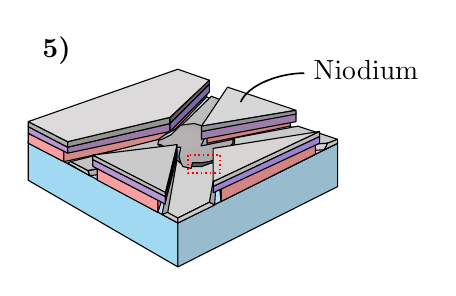
\begin{tikzpicture}



  \draw[line join=bevel, fill=cyan!89!violet!40] (0,1.17) -- (0,0.68) -- (1.9,-0.42) -- (1.9,0.138) -- cycle;
  \draw[line join=bevel, fill=cyan!87!purple!34!lightgray] (1.9,0.138) -- (3.93,1.15) -- (3.93,0.6) -- (1.9,-0.42) -- cycle;

  \draw[fill=cyan!91!purple!31, line join=bevel, draw opacity=1, fill opacity=1] (0,1.159) -- (1.9,1.864) -- (3.93,1.151) -- (1.9,0.139) -- cycle;

  \draw[fill=lightgray!83, line join=bevel] (2.472,1.002) -- (2.523,1.1) -- (2.529,1.2) -- (3.425,1.367) -- (3.929,1.2) -- (3.799,1.15) -- (3.22,1.116) -- cycle;

  \draw[fill=lightgray!97, line join=bevel] (3.929,1.2) -- (3.929,1.15) -- (3.761,1.068) -- (3.8,1.15) -- cycle;
  \draw[fill=white!95!red!69!gray, line join=bevel] (3.761,1.068) -- (3.12,1.025) -- (3.278,1.134) -- (3.544,1.134) -- (3.8,1.15) -- cycle;
  \draw[fill=lightgray!96!gray] (2.326,1.747) -- (1.938,1.369) -- (2.1,1.378) -- (2.2,1.343) -- (2.448,1.7) -- cycle;
\draw[fill=lightgray!81!darkgray, line join=bevel] (2.3,0.4) -- (2.367,0.365) -- (2.4,0.853) -- (1.817,0.853) -- (1.7,0.246) -- (1.8,0.269) -- (1.86,0.8) -- (2.349,0.8) -- cycle;
  \draw[fill=lightgray!71, line join=bevel] (1.891,0.95) -- (1.979,0.916) -- (2.164,0.916) -- (2.3,0.944) -- (2.4,0.95) -- (2.3,0.4) -- (1.9,0.2) -- (1.769,0.257) -- cycle;
  \draw[fill=lightgray!80, line join=bevel] (1.769,0.272) -- (1.7,0.246) -- (1.9,0.138) -- (1.9,0.2) -- cycle;
  \draw[fill=lightgray!82, line join=bevel] (2.3,0.4) -- (2.367,0.365) -- (1.9,0.138) -- (1.9,0.2) -- cycle;
  \draw[line join=bevel, fill=pink!97!teal!84!red, fill opacity=1] (0,1.276) -- (0,1.15) -- (0.451,0.916) -- (0.453,1.05) -- cycle;

  \draw[line join=bevel, fill=lightgray!95!pink!71!red, fill opacity=1] (0.453,1.05) -- (0.453,0.916) -- (1.748,1.2) -- (1.748,1.325) -- cycle;
  \draw[line join=bevel, fill=gray!86!white!77!red, fill opacity=1] (2.27,1.8) -- (2.267,1.74) -- (1.748,1.2) -- (1.748,1.325) -- cycle;
  \draw[fill, shade, shading=ball, ball color=blue!74!green!32] (1.742,1.05) -- (1.579,1.15) -- (1.742,1.261) -- (1.934,1.365) -- (2.1,1.378) -- (2.362,1.286) -- (2.617,1.216) .. controls (2.628,1.156) and (2.617,1.1) .. (2.582,1.05) -- (2.633,0.874) -- (2.324,0.9) -- (2.2,0.853) -- (2.1,0.853) -- (1.965,0.874) -- cycle;
  \draw[fill=gray!97!red!60, fill opacity=0.95, line join=bevel] (1.579,1.134) -- (1.678,1.134) -- (1.753,1.09) -- (1.938,1.1) -- (1.914,0.982) -- (1.938,0.9) -- (1.965,0.854) -- (2.07,0.83) -- (2.085,0.902) -- (2.193,0.902) -- (2.3,0.918) -- (2.4,0.951) -- (2.6,1.151) -- (2.6,1.2) -- (2.193,1.115) -- (2.3,1.344) -- (2.106,1.401) -- (1.938,1.38) -- (1.816,1.259) -- (1.7,1.2) -- (1.6,1.171) -- cycle;

  \draw[fill=gray!98!red!47, line join=bevel]  (0.757,0.803) -- (1.845,1.024) -- (1.646,1.133) -- (1.66,1.2) -- (0.537,0.916) -- cycle;
  \draw[fill=lightgray!78, line join=bevel] (0.76,0.801) -- (0.782,0.737) -- (0.5,0.9) -- (0.537,0.917) -- cycle;
  \draw[fill=lightgray!91!black, line join=bevel] (0.76,0.8) -- (0.782,0.737) -- (1.236,0.8) -- (1.174,0.882) -- cycle;
  \draw[line join=bevel, fill=cyan!51!magenta!81!orange, fill opacity=1] (0.5,1.1) -- (0.5,1.024) -- (1.8,1.3) -- (1.8,1.4) -- cycle;
  \draw[line join=bevel, fill=purple!80!magenta!59!cyan, fill opacity=1] (2.3,1.9) -- (2.3,1.8) -- (1.8,1.3) -- (1.8,1.4) -- cycle;
  \draw[line join=bevel, fill=white!87!magenta!72!blue, fill opacity=1] (0,1.361) -- (0,1.276) -- (0.5,1.024) -- (0.5,1.1) -- cycle;
  \draw[line join=bevel, fill=gray!99!brown!85, fill opacity=1] (0.5,1.17) -- (0.5,1.1) -- (1.8,1.4) -- (1.8,1.479) -- cycle;
  \draw[line join=bevel, fill=gray!98!red!76!black, fill opacity=1] (2.3,1.955) -- (2.3,1.904) -- (1.8,1.4) -- (1.8,1.474) -- cycle;
  \draw[line join=bevel, fill=lightgray!91!black, fill opacity=1] (0,1.425) -- (0,1.361) -- (0.5,1.1) -- (0.5,1.17) -- cycle;

  \draw[line join=bevel, fill=pink!97!teal!84!red, fill opacity=1] (0.876,0.828) -- (0.876,0.683) -- (1.646,0.272) -- (1.646,0.429) -- cycle;
  \draw[line join=bevel, fill=lightgray!90!black!70!red, fill opacity=1] (1.858,1) -- (1.86,0.937) -- (1.646,0.272) -- (1.646,0.429) -- cycle;
  \draw[line join=bevel, fill=white!87!magenta!72!blue, fill opacity=1] (0.82,0.944) -- (0.82,0.857) -- (1.742,0.376) -- (1.742,0.473) -- cycle;
  \draw[line join=bevel, fill=blue!70!orange!56, fill opacity=1] (1.891,1.05) -- (1.891,0.975) -- (1.742,0.4) -- (1.742,0.477) -- cycle;

  \draw[line join=bevel, fill=lightgray!97!black, fill opacity=1] (0.82,1) -- (0.82,0.943) -- (1.742,0.473) -- (1.742,0.531) -- cycle;
  \draw[line join=bevel, fill=gray!88!black, fill opacity=1] (1.891,1.133) -- (1.891,1.05) -- (1.742,0.473) -- (1.742,0.531) -- cycle;

  \draw[line join=bevel, fill=lightgray!83] (0.82,1) -- (1.891,1.133) -- (1.742,0.526) -- cycle;
  \draw[fill=lightgray!99!red!56, line join=bevel] (0,1.425) -- (0.5,1.17) -- (1.8,1.479) -- (2.3,1.95) -- (1.9,2.09) -- cycle;
  \draw[fill=lightgray!99!gray!69!red, line join=bevel] (2.448,0.644) -- (2.448,0.41) -- (3.647,1.01) -- (3.646,1.235) -- cycle;
  \draw[fill=pink!97!teal!84!red, line join=bevel] (2.448,0.42) -- (2.426,0.636) -- (2.448,0.706) -- (2.448,0.6) -- cycle;

  \draw[fill=white!79!darkgray, line join=bevel] (2.532,1.863) -- (2.2,1.367) -- (3.4,1.569) -- cycle;

  \draw[fill=lightgray!96!darkgray, line join=bevel] (3.7,1.3) -- (3.7,1.235) -- (2.35,0.6) -- (2.349,0.664) -- cycle;
  \draw[fill=red!96!teal!34!lightgray, line join=bevel] (2.27,1.245) -- (2.27,1.15) -- (3.327,1.368) -- (3.332,1.45) -- cycle;
  \draw[fill=cyan!56!brown!63!magenta, line join=bevel] (2.2,1.3) -- (2.2,1.2) -- (3.4,1.424) -- (3.4,1.537) -- cycle;
  \draw[fill=gray!96!blue!84, line join=bevel] (2.2,1.368) -- (2.2,1.3) -- (3.4,1.52) -- (3.4,1.568) -- cycle;
  \draw[fill=blue!68!orange!58, line join=bevel] (3.7,1.235) -- (3.7,1.15) -- (2.35,0.522) -- (2.349,0.6) -- cycle;
  \draw[fill=gray!95!red!32, line join=bevel] (2.349,0.664) -- (2.349,1.085) -- (3.7,1.3) -- cycle;
  


  \draw[red, densely dotted, semithick] (2.029,1.002) rectangle (2.437,0.771);
  \node at (4.29,2.08) {Niodium};
  \draw[semithick, line cap=round] (3.5,2.04) .. controls (3.2,2.04) and (2.8,1.9) .. (2.7,1.677);

  \node at (0.36,2.325) {\textbf{5)}};
\end{tikzpicture}